\chapter{A graph-based approach to diploid genome assembly}
Constructing high-quality haplotype-resolved \textit{de novo} assemblies of diploid genomes is important to reveal the full extent of structural variation and its role in health and disease.
Current assembly approaches often put the two sequences into one haploid consensus sequence and, therefore, fail to capture the diploid nature of the organism under study.
Thus, coming up with an assembler which is able to produce accurate and complete diploid assemblies, while being resource-efficient with respect to sequencing costs, 
is a key challenge to be addressed by the bioinformatics community.\\

In this chapter, we present a novel graph-based approach to diploid assembly, which integrates accurate Illumina data and long-read Pacific Biosciences (PacBio) data.
We demonstrate the effectiveness of our method on a pseudo-yeast diploid genome and show that we require as little as 50$\times$ coverage Illumina data 
and 10$\times$ PacBio data to generate accurate and complete assemblies.
Additionally, we show that our approach has the ability to detect and phase structural variants.\\


\section{Introduction}
% Determining the two genome sequences per chromosome of diploid organisms is important.
% Separate determination of the two haplotype sequences can in principle avoid genotyping errors in complex regions of the genome caused by incorrect models of variants at nearby sites being independent.
As introduced in Chapter~\ref{ref:chp1}, the process of assembling the two genome sequences from sequencing reads in a haplotype-aware manner is known as \textit{diploid} or \textit{haplotype-aware genome assembly} and the generated assemblies are called ``haplotigs''.
However, the characteristics of next generation sequencing (NGS) reads are variable, short length and have low error rates; therefore, solving the diploid assembly problem is fundamentally challenging.
Additional challenges inherent in the genome assembly problem include dealing with short and long genomic repeats, handling other rearrangements present in the genome, and scaling efficiently considering input size, genome size, and hardware availability.

Across the short, long, and hybrid categories, most current assemblers \citep{sohn2016present, simpson2015theory} require collapsing the two genome sequences of a diploid sample into a single haploid ``consensus'' sequence (or primary contig). 
The consensus sequence is obtained by merging together the distinct alleles at heterozygous regions into a single allele, and therefore losing a lot of information.
The resulting haploid de novo assembly does not represent the true characteristics of the diploid input genome. 

To generate diploid assemblies for heterozygous genomes, there are two standard linear approaches; 
one uses haploid contig sequences \citep{chin2016phased, pendleton2015assembly, seo2016novo, mostovoy2016hybrid}, 
while the other partitions the reads while using the reference genome as a backbone \citep{Glusman2014, martin2016whatshap, chaisson2017multi}.
% \todo{Maybe we should cite the HGSVC preprint. Tobi: I can insert this.}
In both approaches, the reads are first aligned (either to the reference genome or the contigs). Second, variants such as SNVs are detected based on the aligned reads. 
Finally, the detected variants are phased using long reads from a same or different sequencing technology.

For both reference-guided and contig-based assembly, this third step---solving the phasing problem---has been formulated as the minimum error correction (MEC) optimization problem \citep{lippert2002algorithmic,Cilibrasi2007}.
There are several disadvantages to reference-guided assembly; for example, the reads are initially aligned to the reference genome and therefore the process contains a reference bias. 
The sequences or structural variations that are specific to the genome are not detected by using these approaches. 
Thus, we can not find the cause of the disease, which is actually associated with this structural variant in the genome.

However, there are also several reasons why the set of sequences/contigs produced by contig-based assembly is not ideal.
First, the contigs produced by assemblers ignore the heterozygous variants in complex regions, opting instead to break contiguity to express even moderate complexity. 
Second, the contigs do not capture end-to-end information in the genome; the ordering or relationships between contigs are required in order to generate end-to-end chromosomal-length assemblies.
% \todo{TM: I do not understand this sentence. Can you explain / make this more clear?}
% \sgnote{Done.}

Some newer diploid assembly methods include \cite{weisenfeld2017direct}, where 10x Genomics linked read data is used to determine the actual diploid genome sequence. 
Their approach is based on de Bruijn graphs and applies a series of graph simplifications, in which simple bubbles are detected and phased by using (short) reads that stem from the same (long) input molecule, which is determined through barcoding.
There is also a recent study by \cite{chin2016phased}, who follows a linear phasing approach to generate diploid assemblies (\textit{haplotigs}) for diploid genomes by using PacBio reads.

\paragraph{Contributions.}
We propose a graph-based approach to generate haplotype-aware assemblies of single individuals.
Our contribution is twofold. First, we propose a hybrid approach to integrate accurate Illumina and long PacBio reads to generate diploid assemblies. 
The Illumina reads are used to generate an assembly graph that serves as a backbone for subsequent PacBio-based steps.
Second, we generalize the diploid assembly problem to encompass constructing the diploid assembly directly from the underlying assembly graph.
The two genome sequences can be seen as two paths over the regions of heterozygosity in the assembly graph.
We make some first steps towards performing read-based phasing on graphs.

Figure~\ref{fig:ex_graph_approach} demonstrates the conceptual advantages of our graph-based approach over the Falcon Unzip method.
Consider four SNVs separated by two large SVs and there are four reads spanning these variants.
Falcon Unzip can not phase the central region because the reads $r_3$ and $r_4$ do not cover any SNVs, resulting in incomplete haplotigs.
In contrast, graph-based approaches attempt to detect all types of SVs and phase all of them.

% Based on the above example, we observe that it is possible to deliver complete and contiguous haplotigs using assembly graph-based approach.
\begin{figure}[t!]\centering
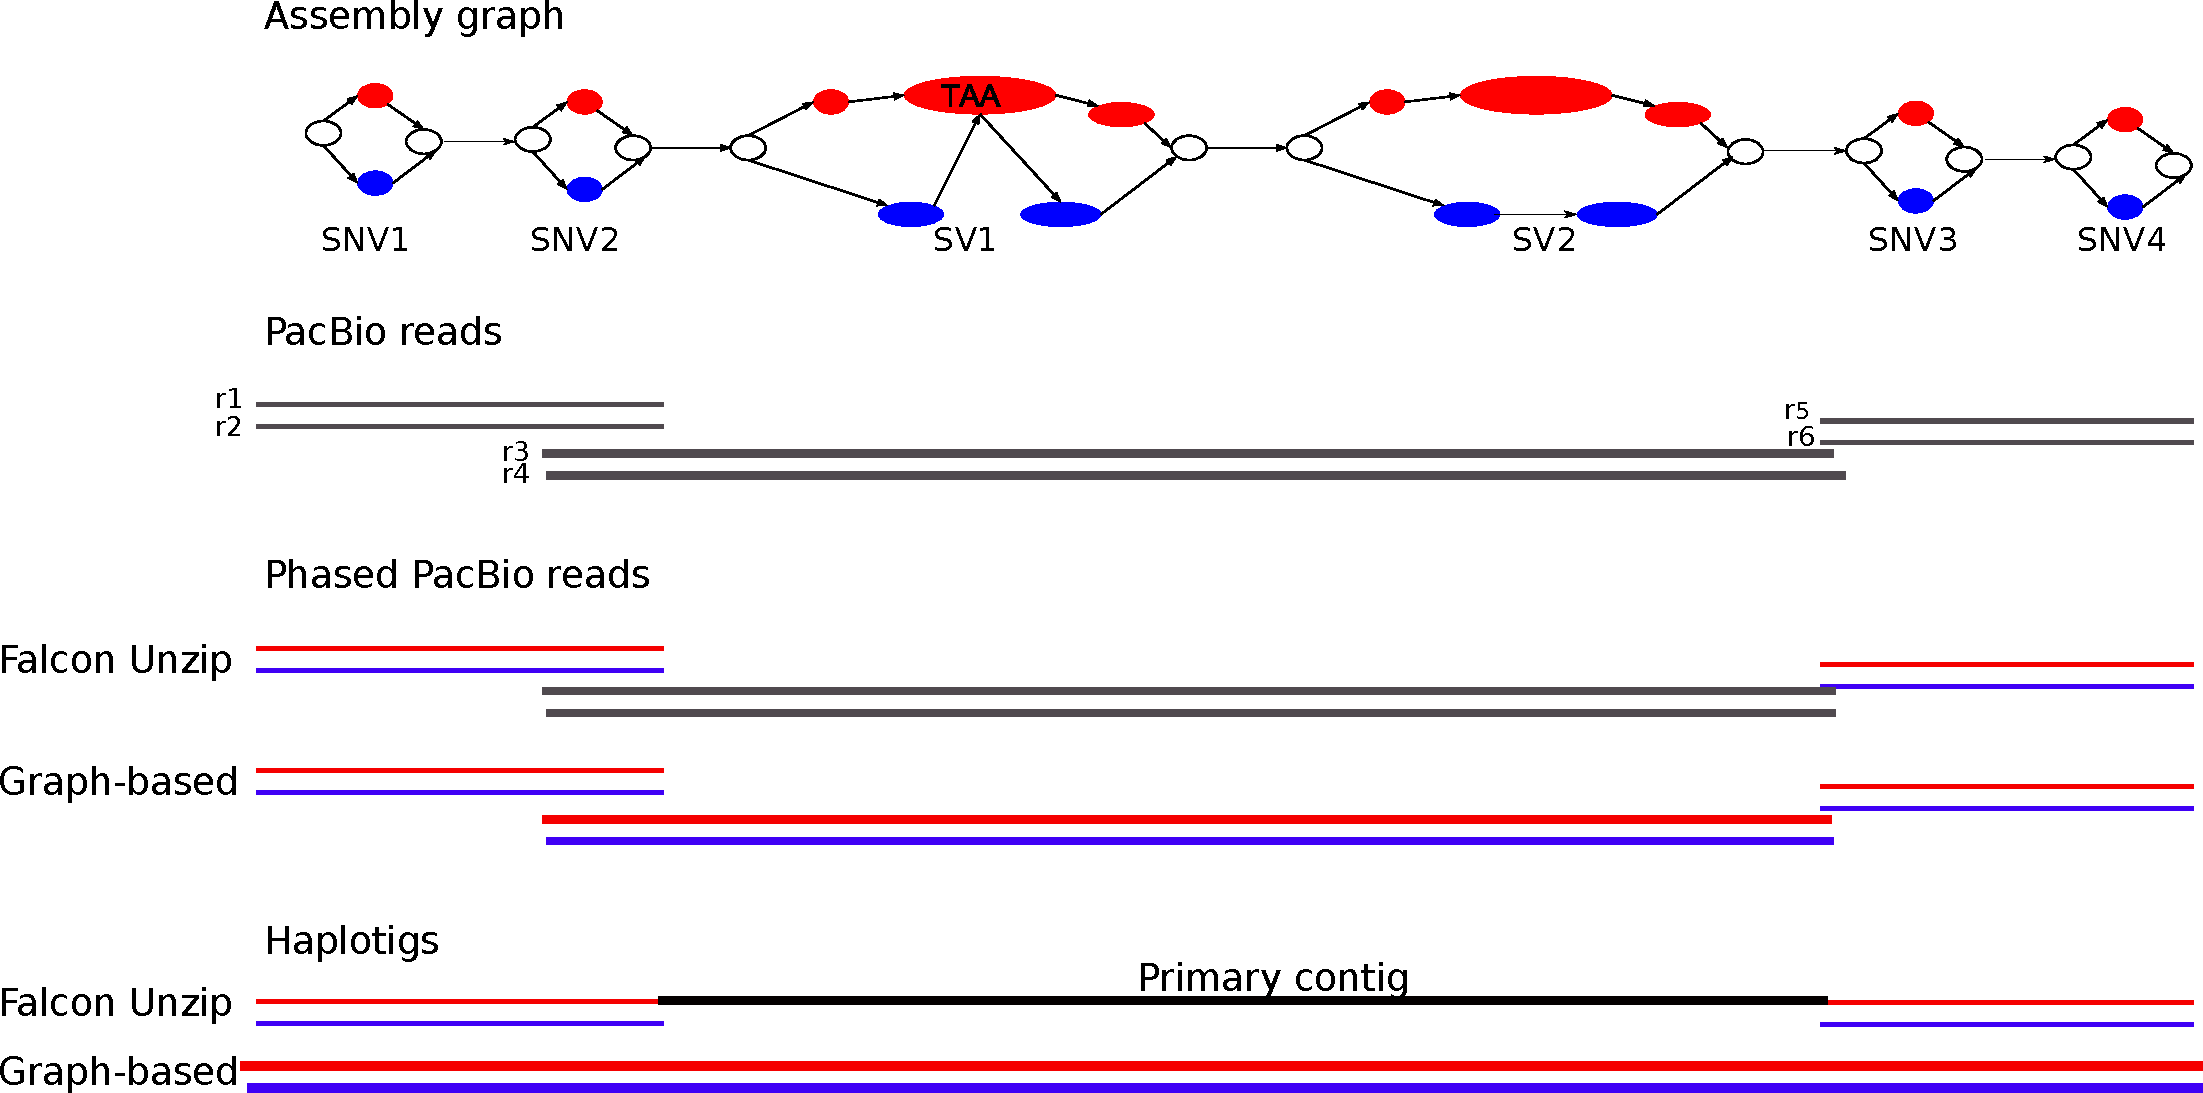
\includegraphics[width=\columnwidth]{ex_graph_approach.pdf}
\caption{Input: an assembly graph (top) (consisting of four SNVs and two SVs) and the PacBio reads $r_1, r_2, r_3, r_4, r_5, r_6$ (gray). 
Output: the phased reads (colored in blue and red) and haplotigs (bottom) using Falcon Unzip and our graph-based approach. Our graph-based phases central region, contrarily, Falcon Unzip does not.  }
\label{fig:ex_graph_approach}
\end{figure}

% Phasing using an assembly graph has several advantages over other approaches. For example, it is possible to phase larger blocks at once, because paths in an assembly graph can span multiple variants.
% Moreover, it is easier to detect large structural variants, such as translocations and other rearrangements, in an assembly graph.
% The structural variants are reflected by bubbles in an assembly graph. The bubbles are defined as a set of disjoint paths that share the same start and end nodes. 
% Figure~\ref{fig:ex_sv} illustrates how such bubbles can represent both small variants (SNVs and indels up to 50 base pairs in length) and larger structural variants.
% The graph-based approach provides a way to both accurately detect all types of structural variation and perform further downstream analyses.
% Figure~\ref{fig:ex_graph_approach} shows the conceptual advantage of our graph-based approach over contig-based methods such as Falcon Unzip.
% Consider four SNVs separated by two large SVs and there are four reads spanning these variants.
% Out of those reads, the two reads $r_3$ and $r_4$ span the two SVs, but do not cover any of the two SNVs.
% In this case, Falcon Unzip generates a primary contig that spans from one end to the other, but generates incomplete and fragmented haplotigs (phased primary contigs in the language of Falcon Unzip).
% % Since we are interested in haplotypes, we talk in the language of \textit{haplotigs} in the rest of the article.
% % \todo{Commented out a sentence that disrupted the flow. Better define ``haplotig'' already above?}.
% % \sgnote{I added it in the second para of Introduction.}
% In contrast, our graph-based approach attempts to phase across all types of variation, including SVs, in order to produce end-to-end haplotigs.
% Therefore, the graph-based approaches are powerful to deliver more complete and contiguous haplotigs.
% In Section~\ref{sec:phasing} we discuss in detail how we can phase these bubbles using graph-based approach. 

We demonstrate the feasibility of our approach by performing a haplotype-aware de novo assembly of a whole pseudo-diploid yeast (SK1+Y12) genome.
We show that we generate accurate, contiguous, and correctly phased diploid genomes.
Through analysis of different coverage levels, we demonstrate that we require only 50$\times$ short-read coverage and as little as 10$\times$ long-read coverage data to generate diploid assemblies.
This illustrates that our hybrid strategy is a cost-effective way of generating haplotype-resolved assemblies.
% Our hybrid assembler, which operates on both long reads (with low coverage) and short reads (with higher coverage), has the potential to generate high-quality assemblies at reduced cost.
Finally, we show that we successfully detect and phase large structural variants.


% \begin{figure}[t!]\centering
% 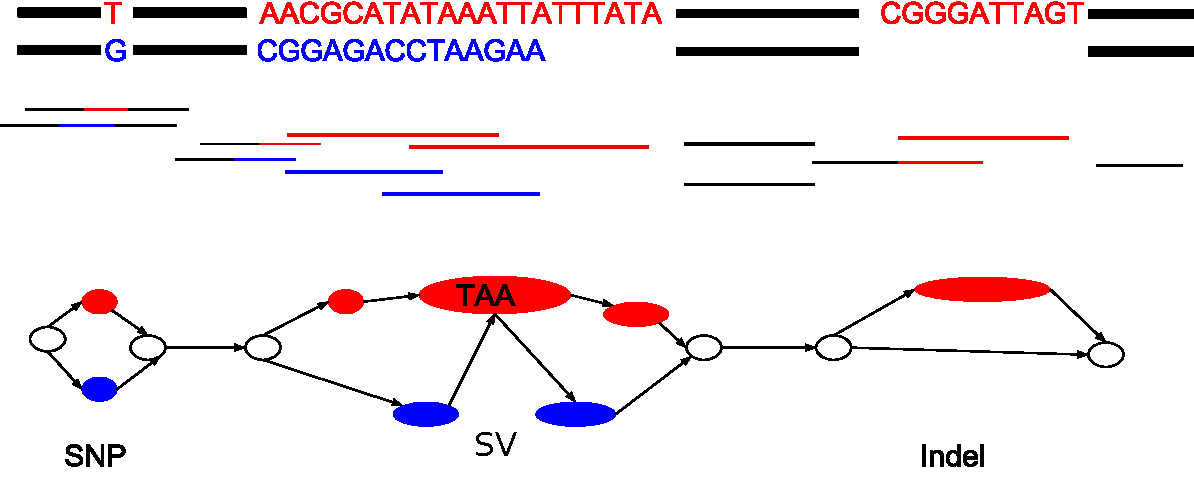
\includegraphics[width=\columnwidth]{ex_sv.pdf}
% \caption{Based on reads (middle) from the two sequences (top), the bubbles in the graph (bottom) show three different heterozygous variations; the first one is an SNV, the second one is an SV, and the third one is an indel. }
% \label{fig:ex_sv}
% \end{figure}

% \begin{figure}[t!]\centering
% 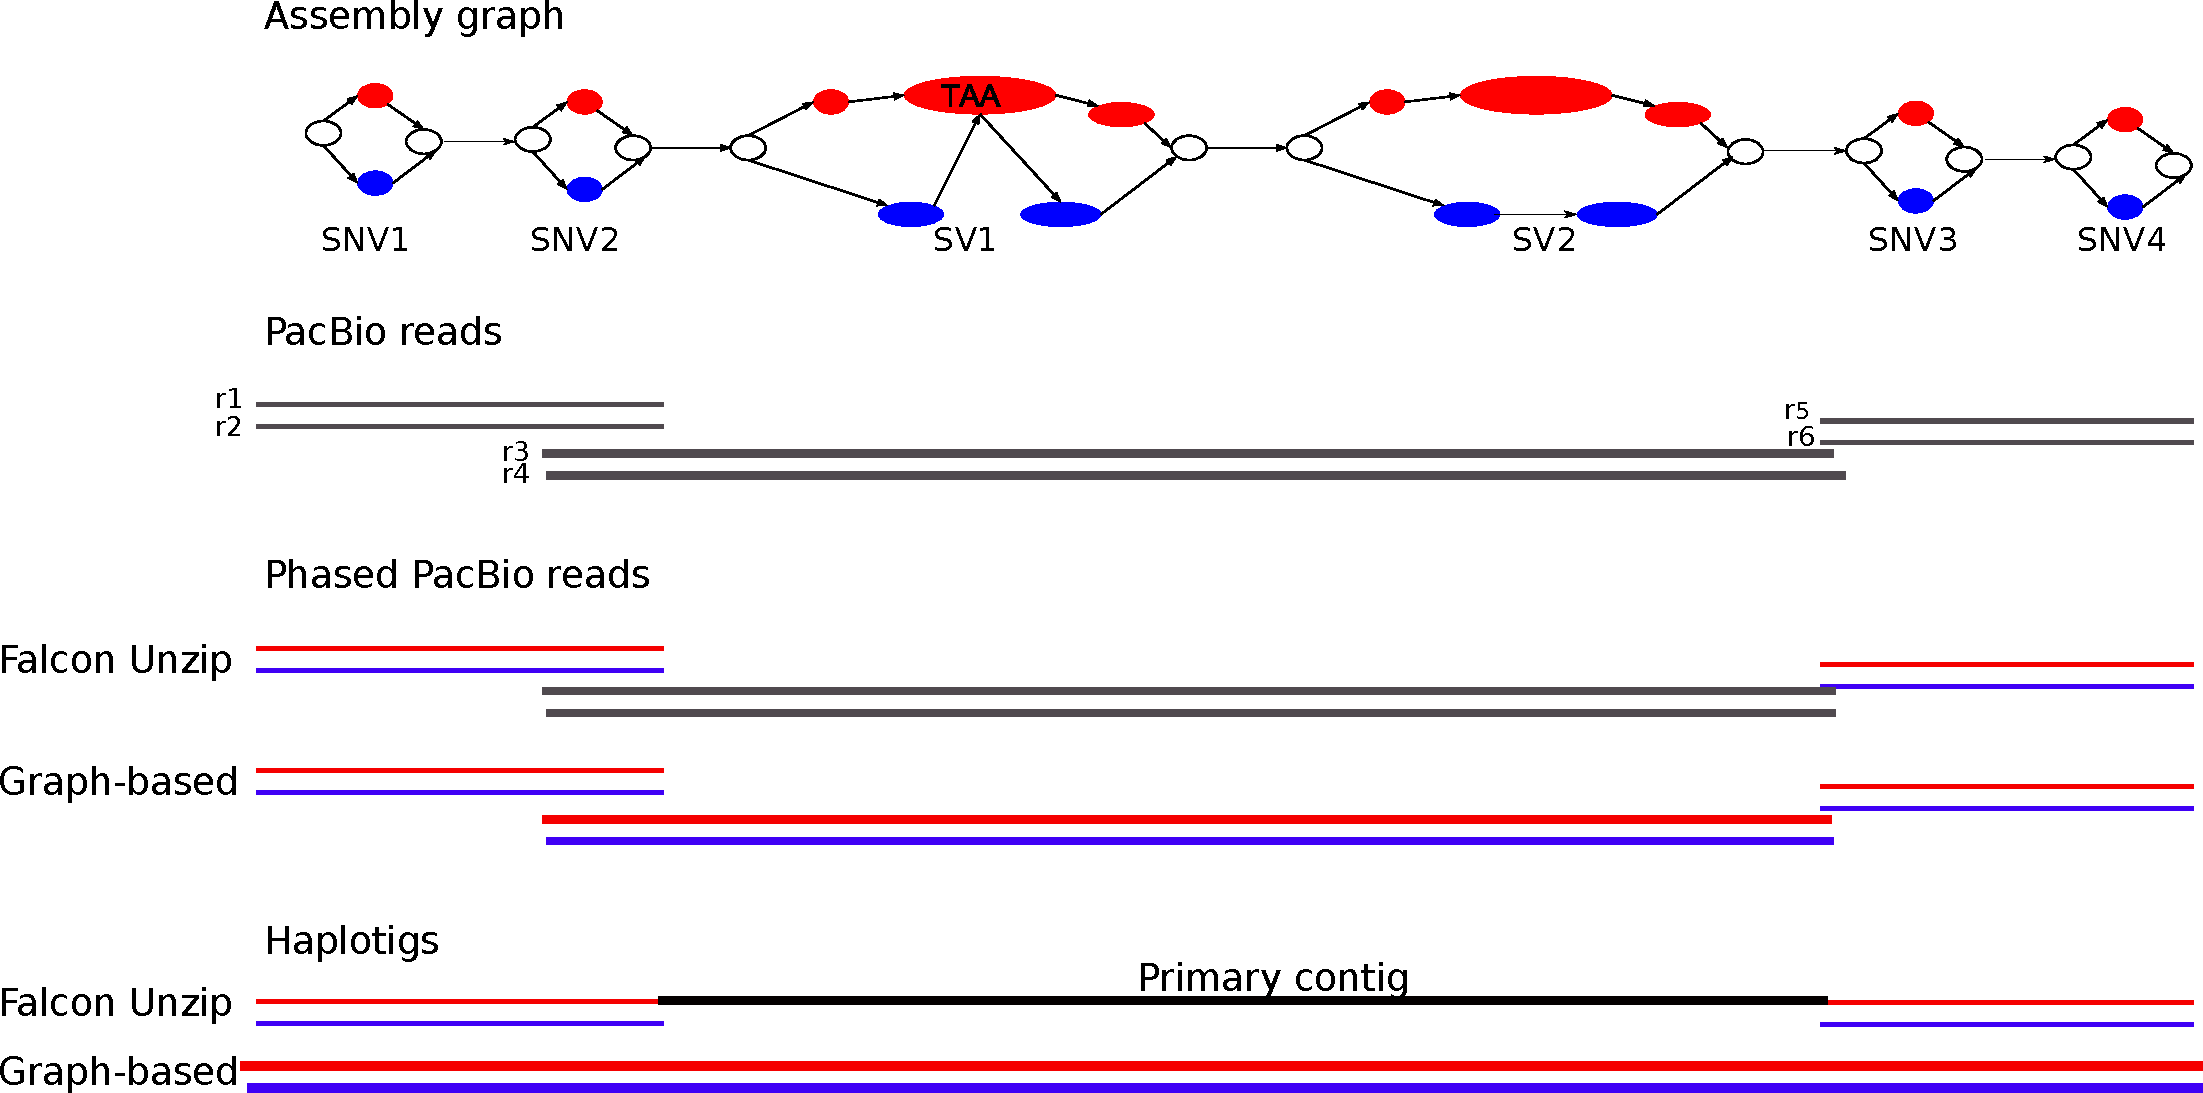
\includegraphics[width=\columnwidth]{ex_graph_approach.pdf}
% \caption{Input: an assembly graph (top) (consisting of four SNVs and two SVs) and the PacBio reads $r_1, r_2, r_3, r_4, r_5, r_6$ (gray). Output: the phased reads (colored in blue and red) and haplotigs (bottom) using Falcon Unzip and our graph-based approach. 
% Our graph-based approach delivers end-to-end haplotigs. Contrarily, Falcon Unzip does not phase the central section, which does not contribute to the total haplotig size.}
% \label{fig:ex_graph_approach}
% \end{figure}
% https://dl.acm.org/citation.cfm?id=322075
% https://www.ncbi.nlm.nih.gov/pmc/articles/PMC5411783/
% http://journals.plos.org/plosone/article?id=10.1371/journal.pone.0019175
\section{Further related work}
The assembly problem was initially formalized as the shortest common super-string problem \citep{maier1978complexity} to generate consensus sequence.
The SCS problem turned out to be NP-hard, thus \cite{tarhio1988greedy} followed the greedy approach to find an approximate solution to solve the assembly problem.
The basic idea of this approach is to combine the two reads that overlap to a maximum extent in terms of length or base quality estimates.
This process is repeated until a predefined minimum quality threshold is reached.

The initial genome assemblers \citep{sutton1995tigr, Green99phrapdocumentation} were based on the greedy strategies and have been used during the Human Genome Project.
Greedy approaches were also explored for datasets generated by second-generation DNA sequencing technologies \citep{warren2006assembling, jeck2007extending}.

The major disadvantage of these greedy approaches is that the shortest common super-string problem neglects an essential feature of complex (e.g.,
vertebrate) genomes: repeats. This has led to the invention of graph-based models for sequence assembly to handle repeats and other complex genomes.
Graph-based models form the basis of most current genome sequence assemblers. 
As introduced in Chapter~\ref{ref:chp1}, there are basically two types of graph models such as de Bruijn and OLC-based string graphs.
Over the last few years, a lot of effort has been devoted to improving the graph based assemblers. 

The Edena assembler followed the string graph approach for short-read sequencing data \citep{hernandez2008novo}. 
To efficiently construct the string graph, several assemblers were developed using the FM index \citep{simpson2010efficient}, 
which led to memory-efficient assemblers for large genomes \citep{li2012exploring, simpson2012efficient}. The latest version of SGA implemented Bloom filter to reduce the running time.
Furthermore, several fast string graph construction algorithms were developed \citep{dinh2011memory, gonnella2012readjoiner, ben2014string}.
 
\begin{figure}[t!]\centering
\includegraphics[width=\columnwidth]{{cropped_falcon-unzip}.pdf}
\caption{(a) An initial assembly graph is constructed by FALCON by error-correcting the reads. 
The bubbles are collapsed into a consensus sequence ``primary contig''.
(b) Heterozygous SNPs  are identified and phased, thus haplotype of reads is identified. (c) The phased reads are used to incorporate the haplotype-fused path into the initial assembly graph, thus finally a set of primary contigs and associated haplotigs are generated.
Figure from paper ``Phased diploid genome assembly with single-molecule real-time sequencing''.}
\label{fig:falcon_unzip}
\end{figure}
In the direction of de Bruijn graph, there were also quite a lot of effort involved.
The ABySS assembler \citep{simpson2009abyss} introduced a representation of
the graph as a hash table of k-mers, with each k-mer storing a byte representing the presence or absence of its eight possible
neighboring k-mers. This representation helped in computational gain by allowing distribution of the hash table across a cluster
of computers. In recent years, the use of Bloom filters \citep{bloom1970space} has been gaining popularity by representing a set of k-mers.
The Bloom filter was first applied to k-mer counting by \cite{melsted2011efficient}. 
The FM-index data structure \cite{ferragina2000opportunistic}, which was basically designed for mapping reads to the reference genome, was also used for
sequence assembly. 
The FM-index, with slight modifications, has been recently used for representing de Bruijn graphs \citep{bowe2012succinct, rodland2013compact}.
The main point that only a fraction of k-mers need to be directly stored as vertices was observed by \cite{ye2012exploiting}. A similar
technique was used to improve the memory consumption of the popular SOAPdenovo assembler \citep{luo2012soapdenovo2}.
All steps in SOAPdenovo pipeline can be customized according to users requirements.

Several algorithms that particularly considered the mate-pair information during assembly have been developed .
 In the works of \cite{butler2008allpaths, bankevich2012spades}, the assembler attempted to enumerate all the paths connecting the endpoints of a mate pair.
The paired de Bruijn graph \citep{medvedev2011paired} approach modified the de Bruijn graph
structure to implicitly encode the mate-pair information, thereby simplifying, resolving repeats and scaffolding of the graph based on the mate-pair information.
\paragraph{Long-read assemblers.}
Although these short-read assemblers can generate consensus sequences to span entire chromosomes, they are very fragmented and lack the finer resolution required to improve contig lengths. 
Instead, the biggest gains in contig lengths stem from single-molecule sequencing, which generates long-read datasets.
These long-read technologies such as PacBio and ONT can generate reads longer than Illumina, but have high error rates. 
More specifically, these reads are long enough to cover the most common repeats in both microbial and vertebrate genomes and can therefore generate highly continuous assemblies. 
Subsequent efforts have been devoted to handling long read lengths and high error rates error rates to generate good quality assemblies.
Several assembly tools are specifically designed for long-read PacBio and Nanopore data such as Canu \citep{koren2017canu}, HINGE \citep{kamath2017hinge}, Racon \citep{vaser2017fast}, Falcon \citep{chin2016phased}, and Miniasm \citep{li2016minimap}.

Canu, which is based on Celera Assembler, has been specifically designed for noisy single-molecule sequences.
Canu followed an adaptive overlapping strategy that involved aligning the PacBio reads based on tf-idf weighted MinHash \citep{berlin2015assembling} and constructed a sparse assembly graph.
It was mainly designed to support long-read data, while being efficient in terms of run-time and coverage requirements, and additionally performed repetition and haplotype separation.
Racon corrected assemblies by finding a consensus sequence between reads and the assembly through the construction of partial order alignment (POA) graphs.
After aligning the reads by mapping tools available (e.g. Minimap or Graphmap),
Racon segmented the sequence and found the best alignment between a POA graph of the reads and the assembly.
The HGAP (Hierarchical Genome Assembly Process) pipeline
was developed to assemble PacBio-generated data without requiring correction using short-read
data \citep{chin2013nonhybrid}. HGAP was a hierarchical pipeline; it selected the longest PacBio reads to form the basis
of the assembly and performed their error-correction using multiple sequence alignment. The corrected
long reads were then assembled, and a consensus sequence was generated using the complete data
set. This method often generated single-contig assemblies of bacterial genomes.
The FALCON assembler followed the design of the hierarchical genome assembly process (HGAP) but used more computationally optimized components. 
It used string graph algorithm for genome assembly and being best suited for PacBio reads.
It included several important steps: error correction of raw reads, pre-assembly error correction, overlap filtering, graph construction from overlaps and contig construction from graph.

\paragraph{Hybrid assemblers.}
Besides short and long-read assemblers, the hybrid approaches to combine different sequencing datasets provide another avenue for generating accurate, contiguous and complete assemblies. 
The hybrid assemblers, SPAdes by \cite{bankevich2012spades} and ALLPATHS-LG by \cite{gnerre2011high}, are DBG-based, which constructs the base graph using Illumina data and then scaffold the assemblies using longer, less accurate reads such as PacBio. 
Furthermore, SPAdes also supports ONT data as the long read complement to NGS data. 
Recently, \cite{fan2017hysa} demonstrates that the combination of PacBio and Illumina delivers accurate structural variant calls.

\paragraph{Other technologies.}
An emerging trend to generate accurate, contiguous and complete assemblies is, to combine cost-effective Illumina sequencing dataset with other sequencing techniques. 
One powerful sequencing technique is chromatin conformation capture via proximity ligation and high-throughput sequencing (Hi-C) \citep{lieberman2009comprehensive}. 
This technique involves in generating a paired-read data type (two reads separated by some distance) but from a distribution of sizes that can span mega bases. 
The main advantage of these data sets is in the scaffolding step to connect contigs, which help in generating chromosome-length scaffolds, and phase haplotypes \citep{burton2013chromosome, selvaraj2013whole}. 
Along the similar lines, \cite{rice2017improved} demonstrates on using in vitro reconstituted chromatin and Illumina sequencing to assemble the American alligator genome. 
Another sequencing technique is the barcoding of short reads to tag groups of ``linked reads'' that all originate from a larger, single molecule of DNA. 
For these synthetic long-read data, \cite{weisenfeld2017direct} introduces a new assembler, Supernova, for the de novo assembly of diploid human genomes. 
Additionally, in the latest version of the ABySS assembler, \cite{jackman2017abyss} explores linked reads and optical mapping for improved scaffolding.

In addition to haploid assemblers, there also exists an only available diploid assembler that has the ability to generate diploid assemblies for diploid organisms.  
\paragraph{Diploid assemblers.}
To date, there is only one diploid assembler, Falcon Unzip. It's pipeline is given in Figure~\ref{fig:falcon_unzip}.
Falcon Unzip first constructs a string graph by using PacBio reads and then collapses the bubbles representing divergent regions between homologous sequences (Fig.~\ref{fig:falcon_unzip}a) to generate sets of ``haplotype-fused contigs'' , also called ``primary contigs''. 
Next, Falcon Unzip aligns reads to the primary contigs and then identifies phases of reads using aligned reads over heterozygous SNVs. (Fig.~\ref{fig:falcon_unzip}b). 
Afterwards, Falcon Unzip identifies haplotypes for the genome and phases each read using greedy approach.
Phased reads are then used to assemble haplotigs (Fig.~\ref{fig:falcon_unzip}c) 
that form the final diploid assembly with phased single-nucleotide polymorphisms (SNPs) and structural variants (SVs).
\begin{figure}[t!]\centering
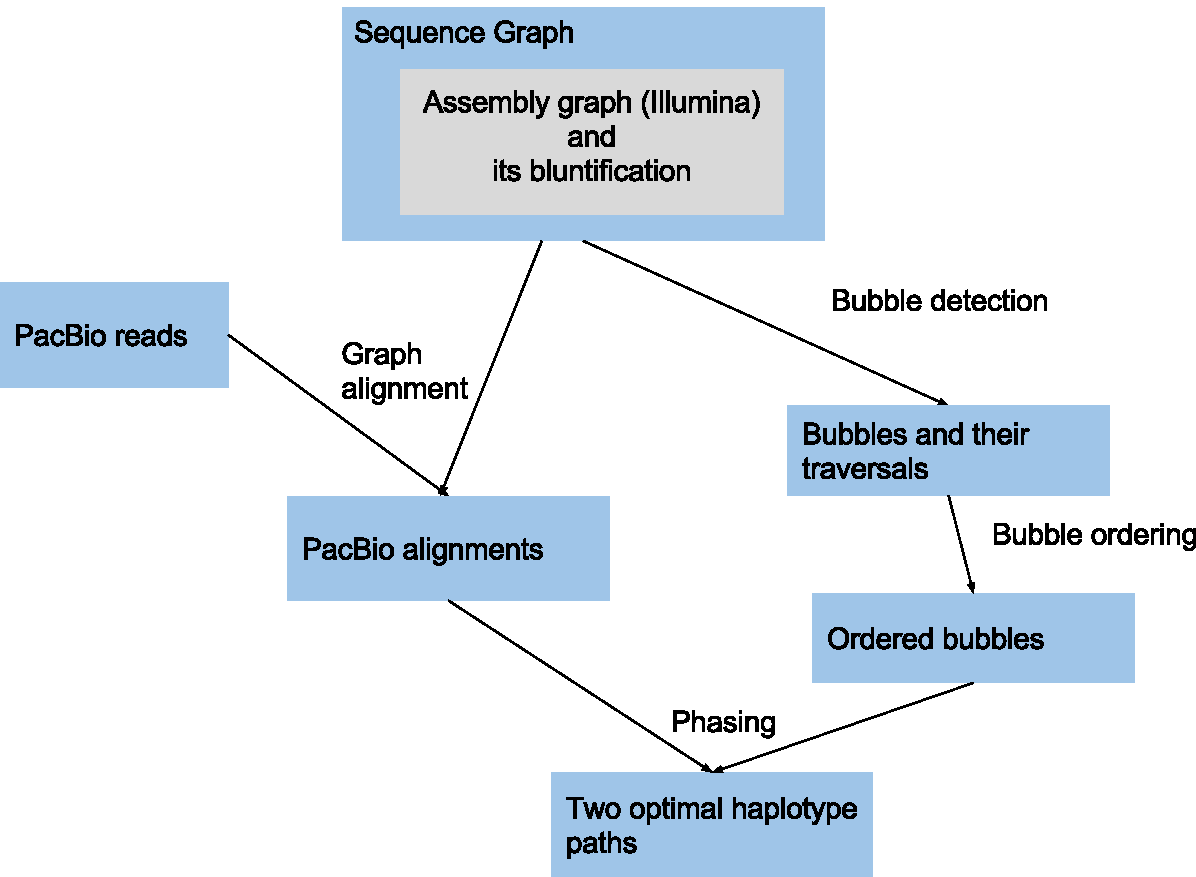
\includegraphics[width=.8\columnwidth]{pipeline.pdf}
\caption{Overview of the diploid assembly pipeline. }
\label{fig:pipeline}
\end{figure}

We now explain the phasing process followed by Falcon Unzip.
The reads are aligned to primary contigs and heterozygous SNPs (het-SNPs) are called by considering signal from sequence alignments.
A simple phasing algorithm based on greedy approach is followed to phase ``chain of SNPs''. 
% Along each contig, the algorithm assigns phasing blocks where ``chained phased SNPs'' can be identified. 
Additionally, the phase to aligned reads can be assigned unambiguously if read covers sufficient heterozygous SNVs.
If a read covers sufficient het-SNPs, then Falcon Unzip assigns a phased tag to each read.
Some reads might not have enough phasing information, thus do not contain phased tag.
For example, if there are not enough het-SNP sites covered by a read, it assigns a special ``un-phased tag'' for each un-phased read.
Furthermore, the initial assembly graph is updated according to phased reads and the haplotigs are generated in a greedy manner using local conservative approach.
% \todo{maybe add example how haplotigs from haplotype fused assembly graph works?}

\section{Diploid assembly pipeline}
In this section, we present a novel diploid assembly pipeline for generating diploid assemblies.
Our assembly workflow uses short read (e.g.\ Illumina) and long read (e.g.\ PacBio) data combinedly, as illustrated in Figure~\ref{fig:pipeline}, and we describe the details of this process in the following.

\subsection{Sequence graph} 
Our first step is to construct a sequence graph using short read data with a low error rate, as provided by the Illumina platform.
% The diploid assembly problem can be modelled using a sequence graph (defined below). We construct the underlying sequence graph using Illumina data.
\begin{definition}[Sequence Graph]
We define a sequence graph $G_s (N_s, E_s)$ as a bidirected graph, consisting of a set of nodes $N_s$ and a set of edges $E_s$.
The nodes $n_i$ are sequences over an alphabet $\mathcal{A} = \{A,C,G,T\}$.
For each node $n_i \in N_s$, its reverse-complement is denoted by $n'_i$.
An edge $e_{i'j}$ connects the nodes $n'_i$ to $n_j$. 
Nodes may be traversed in either the forward or reverse direction, with the sequence being reverse-complemented in the reverse direction. 
% \todo{There was a left/right in the definition at some point. Where did it go (and why)?} \sgnote{Richard and I prefer to write in the language of n and n', it is easier and more mathematical. What do you think? TM: That's ok with me. (Although I disagree that it's more mathematical.)}
\end{definition}

In words, edges represent adjacencies between the sequences of the nodes they connect.
Thus, the graph implicitly encodes longer sequences as the concatenated sequences of the nodes along walks through the graph.

To illustrate this, we consider an example sequence graph $G_s$ in Figure~\ref{fig:wmec}. It consists of a node set $N_s = \{1, 1', 2, 2', 3, 3', \ldots\}$
and an edge set $E_s = \{1 \rightarrow 2', 1 \rightarrow 3' \ldots\}$.

To generate the sequence graph $G_s$, we first employ SPAdes \citep{bankevich2012spades}, which constructs and simplifies a de Bruijn graph, and we subsequently remove the overlaps between the nodes in the resulting graph in a process we call \textit{bluntification}, explained in the Supplement.

\subsection{Bubble detection in sequence graphs} To account for heterozygosity in a diploid genome, we perform bubble detection. The notion of \textit{bubble} we use is closely based on the \textit{ultrabubble} concept as defined by \cite{paten2017superbubbles}. Briefly, bubbles have the following properties:
\begin{itemize}
 \item \textit{2-node-connectivity}. A bubble is bounded by fixed start and end nodes.
 Removing both the start and end nodes disconnects the bubble from the rest of the graph.
 Note that a bubble can be viewed in either orientation.
 If the graph is traversed in one direction, and a bubble is encountered that starts at a node $n_i$  and ends at a node $n'_j$, then that bubble can also be described as the bubble with start node $n_j$ and end node $n'_i$, as it would be encountered when traversing the graph in the opposite direction.
  \item \textit{Directed acyclicity}. A bubble is directed and acyclic.
 \item \textit{Directionality}. All paths through the bubble flow from start to end.
 \item \textit{Minimality}. No vertex in the bubble other than the start node $n_i$ (with proper orientation) forms a pair with the end node $n'_j$ (with proper orientation) that satisfies the above properties. Similarly, no vertex in the bubble other than $n'_j$ forms such a pair with $n_i$.
%  \todo{Reword to avoid ``Only the smallest possible bubble ... is a bubble'' (because larger structures are no bubbles)}
\end{itemize}

A bubble can represent a potential sequencing error or genetic variation within a set of homologous molecules.
We represent bubbles as collections of alternative paths.

\begin{definition}[Path] We define path $a_i$ as a linear ordering of nodes $a_i= n_1, \ldots n_m$. 
% \todo{Why start from a complemented node $n'_1$?}
\label{def:allele-path}
\end{definition}

A bubble is a collection of paths with the same start and end node and can be defined as follows:
\begin{definition}[Bubble]
Formally, a bubble is represented as a collection of allele paths
 $l_k= \{a_1,a_2 \ldots\}$
 where 
 \[a_1=(n_1, n_2, \ldots n_m), a_2=(n_1, n_3 \ldots n_m)\] and so on. 
\end{definition}


For example, Figure~\ref{fig:wmec} shows a set of two bubbles $L=\{l_2, l_1\}$, and the set of allele paths for the
% \todo{TM: did you define ``complex bubble'' already?} 
bubble $l_2$ is $\{a_1, a_2, a_3\}$,
where $a_1 = (6, 7', 8', 11')$, $a_2 = (6, 9', 11')$, $a_3=  (6, 10, 11')$.

\subsection{PacBio alignments} 
For phasing bubbles, we consider long reads from third generation sequence technologies such as PacBio.
We align these long reads to the sequence graph $G_s$ to generate paths through the graph.
We perform graph alignment using a banded version of the algorithm described by \cite{rautiainen2017aligning}, which is a generalization of semi-global alignment to sequence-to-graph alignment\footnote{\url{https://github.com/maickrau/GraphAligner}}.

There are several advantages of aligning PacBio reads to graphs instead of to a reference genome or contigs.
SNPs often occur near larger variants such as insertions and deletions. SNPs are thus often missed in these regions when reads contain large mismatches with respect to the linear sequences they are aligned against. Graph alignment allows the alignment of reads to variants appropriate to each read's phase, and to other types of complex events.

\begin{definition}[Alignment]
We define a set of read alignments as $R=\{r_1, r_2, \ldots, r_j\}$, where each read alignment $r_{j}$ is given by a path of oriented nodes in graph $G_s$, written $r_{j}=(n_1, \ldots, n_m)$.
\end{definition}
For example, in Figure~\ref{fig:wmec}, $R = \{r_1, r_2, r_3, r_4\}$ and the read alignment path $r_1$ can be written as 
$r_1 = (1, 2', 5', 6, 7', 8', 11' ) $


\subsection{Bubble ordering}
The next stage of our algorithm is to obtain an ordering of the bubbles $L=(l_1, l_2, \ldots l_k)$, which we refer to as a \emph{bubble chain}. 
For example, in Figure~\ref{fig:wmec}, $L=(l_1, l_2)$ is a bubble chain.
A general sequence graph $G_s$ is cyclic, due to different types of repeats present in the genome that create both short and long cycles.
Ordering bubbles in such a graph is closely related to resolving repeats, which is a challenging problem.
In this study, we rely on the Canu algorithm \citep{koren2017canu} to provide a bubble ordering by aligning Canu-generated contigs to our sequence graph.
Furthermore, we detect repetitive bubbles---that is, bubbles that would need to be traversed more than once in a final assembly---based on the depth of coverage of aligned PacBio reads, and remove such bubbles.
% \todo{Shilpa, please check these sentence. I reworded them a bit.}
We deem a bubble repetitive if the number of PacBio reads aligned to its starting node is greater than a coverage threshold specified by the user over the genome.
For example, given a 30$\times$ ($=c$) data set and a repeat that occurs 20 ($=r$) times in the genome, then the coverage at the bubble on average is 600 ($=r \cdot c$).

\subsection{Graph-based phasing}
\label{sec:phasing} 
Given a sequence graph $G_s$, ordered bubbles $L$, and PacBio alignments $R$, the goal is to reconstruct two haplotype sequences $\{h_0, h_1\}$, called haplotigs, along each chain of bubbles.
\begin{definition}[Haplotype path]
Formally, a pair of haplotype paths $(h_0, h_1)$ can be defined as two paths through a bubble chain in the sequence graph and denoted as:
\[h_0=(n_s, n_2, \ldots n_e )\]

\[h_1=(n_s, n_3, \ldots n_e )\]

where $h_0$ and $h_1$ may differ at the heterozygous regions defined by bubbles, and $n_s$ and $n_e$ are the start and end of the bubble chain.
% \todo{I'm really confused by these $n'$s. I think we can just use plain $n$s.}
\end{definition}

The two genome sequences can be seen as two walks through the bubbles $L$ in the sequence graph $G_s$ that are consistent with the PacBio alignments $R$.
In maximum likelihood terminology, the goal is to find the most likely haplotype paths given the alignment paths traversing through the bubbles.
For example, in Figure~\ref{fig:wmec}, given bubbles $(l_1, l_2)$ and PacBio alignments $R=\{r_1,r_2,r_3,r_4\}$, the goal is to find two maximum likelihood haplotype paths $\{h_0, h_1\}$ such that each PacBio alignment is assigned to one of the haplotypes. 
% \todo{continue with ``that...'', because you do not just want to find any two paths, but ML ones.}

For a linear chain of bubbles $L$, the task of finding these two haplotype paths is equivalent to picking one allele path per haplotype for each bubble.
% We generate an association between bubbles $L$ and aligned PacBio reads $R$ in the sequence graph $G_s$ in order to encode alignment paths in the form of an allele path in bubbles.
To this end, we note that an alignment path $r_j$ for a given read can be viewed as a sequence of allele paths traversed in consecutive bubbles. 
% stores the information about the allele path $a_i$ in a bubble $l_k$ that the read $r_j$ is aligned.
We represent this association of reads to allele paths in the form of a \emph{bubble matrix} $\mathcal{F}\in\{0,1, \ldots m, -\}^{|R|\times |L|}$, where $|R|$ is the number of reads, $|L|$ is the number of bubbles along a chromosome, and $m = \max_k|l_k|$ is the maximum number of  paths (or alleles) in any bubble $l_k\in L$.
% Please note that the different paths in a bubble corresponds to possible alleles at a genetic variant.
The entry $\mathcal{F}(j,k) \in \{0, 1, \ldots m, -\}$ represents the allele path index in bubble $l_k$ that read $r_j$ is aligned to, where a value of ``$-$'' indicates that the read does not cover the bubble.
% For example, in Figure~\ref{fig:wmec}, the read alignment path $r_1$ traverses an allele path $a_1$ in a bubble $l_1$ and $a_1$ in $l_2$. \todo{TM: The allele paths are not shown in that figure, right? Can we add them?}
In Figure~\ref{fig:wmec}, note that the read alignment path $r_4$ does not cover all the nodes in any of the allele paths in $l_2$ and hence we set the corresponding value $\mathcal{F}(4,2)$ to ``$-$''.
As a result, this read covers only one bubble, which renders it uninformative for phasing, and we do not consider it further.
The remaining phasing-informative reads in Figure~\ref{fig:wmec} are represented as:

\begin{equation}\label{eq:bubble_matrix}
  \mathcal{F}  = \kbordermatrix{
     & l_{1}       & l_{2}  \\
    r_{1}       & 0 & 0 \\
    r_{2}       & 2 & 2 \\
    r_{3}       & 1 & 2 \\
  }
\end{equation}

Corresponding to $\mathcal{F}$, we have a weight matrix $\mathcal{W}\in W^{|R|\times |L|\times m}$. %, where $|R|$ is the number of reads, $|L|$ is the number of bubbles and $m$ is the maximum number of alleles in a bubble $l_k$.
Each entry in $\mathcal{W}(j,k)$ is a tuple storing a weight for each allele, which can for instance reflect ``phred-scaled'' (i.e. $-10\log(p)$) probabilities that the read supports a given allele.
The weight of ``0'' at the $i^\text{th}$ entry in the tuple $\mathcal{W}(j,k)$ encodes that the read $r_j$ is aligned to allele path index $i$ in bubble $l_k$.
The remaining non-zero values in tuple $\mathcal{W}(j,k)$ store the confidence scores of switching the aligned read $r_j$ to other alleles in bubble $l_k$.

For example, the corresponding weight matrix $\mathcal{W}(j,k)$ for $\mathcal{F}$~\eqref{eq:bubble_matrix} is given by:
\begin{equation}\label{eq:weight_matrix}
  \mathcal{W}  = \kbordermatrix{
     & l_{1}       & l_{2}  \\
    r_{1}       & [0,q_1,q_2] &  [0,q_3,q_4]\\
    r_2 & [q_9,q_8,0] & [q_{11},q_5,0] \\
    r_3 & [q_{10},0,q_7] & [q_5,q_6,0] \\
  }
\end{equation}
where the entry $\mathcal{W}(1,1)$ value $[0,q_1,q_2]$ means that the read $r_0$ is aligned to allele $a_0$ at bubble $l_1$.
Additionally, the cost of flipping it to other alleles is $q_1$ for $a_1$ and $q_2$ for $a_2$.
% \todo{We should use different $q$s for each entry.}

We are now ready to present the problem formulation.
The main insight is that solving phasing for bubble chains is similar to solving the phasing problem for multi-allelic SNVs in reference-based haplotype reconstruction.
Therefore, we build on the previous formulation of the Minimum Error Correction (MEC) problem \citep{Lancia2001} and its weighted version (wMEC) \citep{lippert2002algorithmic,Patterson2015} and further adapt it to work on a subgraph consisting of a chain of bubbles, defining the \emph{Minimum Error Correction for graphs} (gMEC) problem.

\begin{figure}[t!]\centering
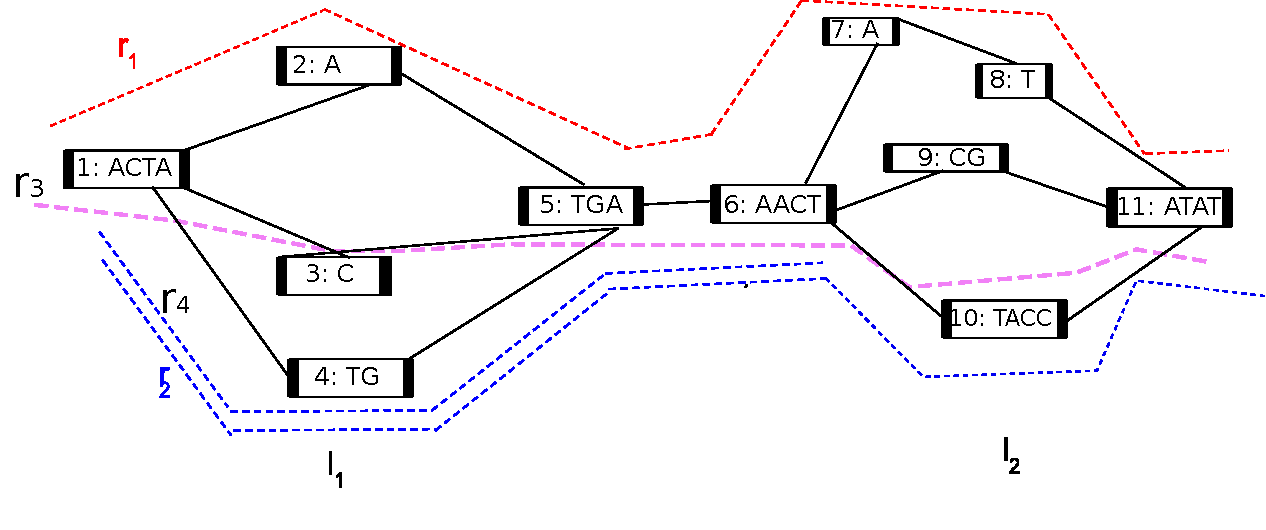
\includegraphics[width=\columnwidth]{wmecfig.pdf}
\caption{For a subgraph of $G_s$, the example shows two bubbles $l_1$ and $l_2$, and their corresponding alleles. Reads $r_1,r_2,r_3,r_4$ traverse the bubbles.}
\label{fig:wmec}
\end{figure}

% \begin{definition}[Distance] 
% The quality of a solution relies on the measure $d(r_1,r_2)$ based on the Hamming distance between any two rows $r_1,r_2$. Formally,
% \[d(p_1,p_2):=\sum_{k=1}^{|L|} \big|\big\{k\,\big|\,r_1(k)\neq -\ \wedge\ r_2(k)\neq -\ \wedge\ r_1(k)\neq r_2(k)\big\}\big|.\]
% \end{definition}
% 
% \begin{definition}[Feasibility]
% A feasible solution to a bubble matrix $\mathcal{F}\in\{a_0, a_1 \ldots a_m, -\}^{|R|\times |L|}$ is a pair of haplotypes $h^0,h^1\in\{a_0, a_1, \ldots a_m\}^M$ such that 
% \[d(h_0,h_1):=\sum_{j=1}^{|R|} \min\{ d(\mathcal{F}(j), h_0), d(\mathcal{F}(j), h_1)\} \]
% and there exists a bi-partition of rows (i.\,e., reads) into two sets such that all pairwise distances of two rows within the same set are zero.
% \end{definition}

\begin{problem}[wMEC for bubble chains (gMEC)]\label{prob:gMEC}
Assume we are given a bubble chain $L=(l_1,\ldots,l_{|L|})$ and a set $R$ of aligned reads $r_j$ that pass through these bubbles, with $\mathcal{F}(j,k)$ indicating the index of the allele in bubble $l_k$ that the alignment of read $r_j$ passes through, or ``$-$'' if it does not pass through $l_k$, and that $\mathcal{W}(j,k,i)$ is the cost of flipping $\mathcal{F}(j,k)$ to new value $i$.  
We want to find two paths through $L$, each of which consists of a sequence of allele indices specifying which allele the path takes in each bubble $l_k$, and then to flip entries of $\mathcal{F}$ such that each row is equal to one of the paths for all non-dash entries while the incurred costs are minimized.
\end{problem}
% For simplicity, we represent the $i^{th}$ element of tuple $\mathcal{W}(j,k)$ as $\mathcal{W}(j,k,i)$.
Note that the wMEC problem constitutes a special case of gMEC, where the input graph is a chain of bi-allelic bubbles.
% In its linear counterpart, wMEC with each entry in $\mathcal{F}(j,k) \in \{0,1\}$ works for bi-allelic cases.
Next, we describe how to solve gMEC via dynamic programming (DP).

In the WhatsHap algorithm \citep{Patterson2015}, wMEC is solved in an exact manner for bi-allelic variants using a dynamic programming approach.
It runs in $\mathcal{O}(2^c\cdot |L|)$ time, where $|L|$ is the number of variants to be phased and $c$ is the maximum physical coverage.
The basic idea is to proceed column-wise from left to right over a set of active reads.
Each read remains active from its first non-dash position to its last non-dash position in $\mathcal{F}$.
In column $k$, we denote the set of active reads as $A(k)$, particularly, $c=\max_{k}\{|A(k)|\}$.
The algorithm now considers all \emph{bipartitions} of $A(k)$, that is, all pairs $B=(P,Q)$ of disjoint sets $P$ and $Q$ such that $P\cup Q=A(k)$.
We fill a DP table column wise and for each column $k$ of $\mathcal{F}$, we fill a DP table column $C(k,\cdot)$ with $2^\abs{A(k)}$ entries corresponding to these bipartitions of $A(k)$.
Each entry $C(k,B)$ is equal to the cost of solving wMEC on the partial matrix consisting of columns $1$ to $k$ of $\mathcal{F}$ such that the bipartition of the full read set $A(1)\cup\ldots\cup A(k)$ \emph{extends} $B$ according to the below definition.
\begin{definition}[Bipartition extension]
For a given set $A$ and a subset $A'\subset A$, a bipartition $B=(P,Q)$ of $A$ is said to \emph{extend} a bipartition $B'=(P',Q')$ of $A'$ if $P'\subset P$ and $Q'\subset Q$.
\end{definition}

Once all entries of the DP table have been computed, the minimum of the last column $\min_B\{C(|L|,B)\}$ indicates the optimal wMEC cost and the optimal bipartition can be obtained by backtracing.
We refer the reader to \cite{Patterson2015} for a more detailed explanation of this algorithm.

\textit{Solving gMEC for bubble chains}. The basic idea is to now extend the dynamic program to consider all possible path-pairs through each bubble. 
In the bi-allelic case, we have only two paths in every bubble and, therefore, there is only one pair of distinct paths.
In the multi-allelic case, we consider all possible path pairs in each bubble.
The goal is to find an optimal pair of paths from the sequence graph $G_s$.
% \todo{what does ``simplified version'' refer to? After repeat removal?} 
Analogously to the WhatsHap algorithm for wMEC, we proceed from left to right using dynamic programming.  
% Assuming we have completed the process up to bubble $l_k$, at bubble $l_{k+1}$ we consider each possible bipartition of all the reads crossing that bubble into two groups.\todo{TM: unclear wording}
% For each bipartition, we find the best pair of alleles and the best assignment at $l_k$.\todo{Can we be more precise here and mention costs in this column vs.\ costs from previous columns?}
% We continue this way until the last bubble $|L|$ and then backtrace to get the two optimal paths.

To explain the dynamic programming algorithm that we use, consider a toy example with the weight matrix~\eqref{eq:weight_matrix}:
\begin{equation}\label{eq:weight_matrix1}
  \mathcal{W}  = \kbordermatrix{
     & l_{1}       & l_{2}  \\
    r_{1}       & [0,10,5] &  [0,5,8]\\
    r_2 & [7,6,0] & [5,2,0] \\
    r_3 & [2,0,4] & [4,3,0] \\
  }
\end{equation}

\textit{DP cell initialization}. Along similar lines as \cite{Patterson2015}, we first compute the local cost incurred by bipartition $B= (R,S)$ in column $k$, denoted $\Delta_C(k,B)$, and later combine it with the corresponding costs incurred in previous columns.
% We write $\mathcal{S}(k,B)$ to denote this set of sets of reads induced by bipartition $B$ in column $k$.
The cost $W_{k,R}^i$ of flipping all entries in a read set $R$ to an allele index $i\in\{0,1,\ldots |l_k|\}$ is given by 
\[W_{k,R}^i = \sum_{j\in R}\iverl \mathcal{F}(j,k)\neq i\iverr\cdot\mathcal{W}(j,k,i),\]
In the same manner, we can compute costs $W_{k,S}^i$ for read set $S$ to an allele index $i$.

To compute the cost incurred by a bipartition in a particular column $k$, we minimize over all possible pairs of alleles in bubble $l_k$.
There are ${|l_k| \choose 2}$ such pairs.
So given the corresponding column vectors $\mathcal{F}(k)$ and $\mathcal{W}(k)$ of the bubble matrix and of the weight matrix, respectively, and the bipartition $B=(R,S)$ of active reads $A(k)$, the cost $\Delta_C(k,B)$ is computed by minimizing over all pairs of alleles
$A = \{(x,y) \in l_k \times l_k | x \ne y, x\textless y\}$:
\begin{equation}\label{eq:dp-cell}
  \Delta_C(k,B)= \min_{(p_0,p_1)\in {A}}\left\{\min\{W_{k,S}^{p_0} + W_{k,R}^{p_1}, W_{k,S}^{p_1} + W_{k,R}^{p_0}\}\right\},
\end{equation}
where the outer minimization considers all allele pairs and the inner minimization considers the two possibilities of assigning those two alleles to the two haplotypes.

   

% \begin{algorithm}
%     \caption{\label{alg:dp-cell}\textsc{DP CELL INITIALIZATION}}
%     \SetKwInOut{Input}{Input}
%     \SetKwInOut{Output}{Output}
%     \Input{The column vectors of the bubble matrix $\mathcal{F}(k)$ and a weight matrix $\mathcal{W}(k)$ of the bubble $k$, and the bipartition $S$ of active reads $R (k)$}
%     \Output{$\Delta_C(k,B)$}
%     All allele-pairs set $A = \{(x,y) \in l_k \times l_k | x \ne y, x\textless y\}$ from bubble $l_k = \{a_1, a_2, \ldots a_m\}$
%     \[\Delta_C(k,B)= \min_{i\in {A}^{\mathcal{S}(k,B)}}\left\{\sum_{S\in\mathcal{S}(k,B)}W_{k,S}^{i}\right\},\]
%     
% \end{algorithm}

\textit{DP column initialization}. 
We initialize the first DP column by setting $C(1,B):=\Delta_C(1,B)$ for all possible bipartitions $B$.
We enumerate all bipartitions in Gray code order, as done previously in \cite{Patterson2015}.
This ensures that only one read is moved from one set to another in each step, facilitating constant time updates of the values $W_{k,S}^i$.

For a variant matrix~\eqref{eq:bubble_matrix} and its corresponding weight matrix~\eqref{eq:weight_matrix1}, the DP column cell for bipartition $B=(R,S)$ is given by
\[\Delta_C(k,(R,S))= \min\big\{W^0_{k,R} + W^1_{k,S}, W^1_{k,R} + W^2_{k,S}, \]
\[W^0_{k,R} + W^2_{k,S}, W^1_{k,R} + W^0_{k,S},\]
\[W^2_{k,R} + W^1_{k,S}, W^2_{k,R} + W^0_{k,S} \big\}\]
Now, plugging values from~\eqref{eq:weight_matrix1} into the above equation for different bipartitions, $\Delta_C(1,.)$ can be filled as follows:
\[
\begin{split}
\Delta_C(1,& (\{r_1,r_2,r_3\},\emptyset)) =\\ & min\{9+0, 16+0, 9+0,16+0, 9+0, 9+0\} = 9 
\end{split}
\]
% \[C(1, (\{r_1,r_2\},\{r_3\})) = \min\{7+2, 16+0, 5+4, 7+0, 16+4, 7+4\} = 7\]
Similarly, we can compute $\Delta_C(1,.)$ for other bipartitions $(\{r_1,r_2\},\{r_3\}),$\\
$(\{r_1,r_3\},\{r_2\}), (\emptyset,\{r_1,r_2,r_3\}), (\{r_3\},\{r_1,r_2\}), (\{r_2\},\{r_1,r_3\})$.

\begin{algorithm}
    \caption{\label{alg:dp-column}\textsc{DP COLUMN INITIALIZATION}}
    \SetKwInOut{Input}{Input}
    \SetKwInOut{Output}{Output}
    \Input{Set $A(1)$ of reads covering bubble $l_1$.}
    \Output{$C(1,.)$}
    \For{ all bipartitions $B$ of column $k$}{
	Compute $\Delta_C(k,B)$ using Equation~\ref{eq:dp-cell} and store in $C(1,B)$.	
    }
\end{algorithm}
Due to the use of the Gray code order, we can perform this operation for one DP column in $\mathcal{O}( {|l_k| \choose 2} \cdot 2^{|A(k)|})$ time.

\textit{DP column recurrence}.
Note that $C(k,B)$ is the cost of an optimal solution of Problem~\ref{prob:gMEC} for input matrices restricted to the first $k$ columns under the additional constraint that the solution's bipartition of the full read set extends $B$.
Since column $k$ lists all bipartitions, the optimal solution to the input matrix consisting of the first $k$ columns would be given by the minimum in that column.
To compute entries in column $C(k+1,\cdot)$, we add up local costs incurred in column $k+1$ and costs from the previous column (see Algorithm~\ref{alg:dp-table}).
To adhere to the semantics of $C(k+1,B)$ described above, only entries in column $k$ whose bipartitions are \emph{compatible} with $B$ are to be considered as possible ``predecessors'' of $C(k+1, B)$.

\begin{definition}[Bipartition compatibility]
For bipartitions $B = (P, Q)$ of $A$ and $B' = (P', Q')$ of $A'$, $B$ and $B'$ are \emph{compatible} if $P \cap A \cap A' = P' \cap A \cap A'$ and $Q \cap A \cap A' = Q' \cap A \cap A'$, denoted by $B \simeq B'$
\end{definition}

For example, consider the second column from~\eqref{eq:bubble_matrix} and~\eqref{eq:weight_matrix1}. Let us compute $C(2,.)$ for different bipartitions using recurrence in Algorithm~\ref{alg:dp-table}:
\[C(2, (\{r_1,r_2,r_3\},\emptyset)) = \min\{9+0, 10+0, 9+0,10+0, 8+0, 8+0\} \]
\[ + \min\{C(1, (\{r_1,r_2,r_3\},\emptyset)\} = 8+9 = 17 \]

To fill DP column $C(2,.)$, we can analogously compute this for the remaining bipartitions $(\{r_1,r_2\},\{r_3\})$,
$(\{r_1,r_3\},\{r_2\})$, $(\emptyset,\{r_1,r_2,r_3\})$, $(\{r_3\},\{r_1,r_2\})$, and $(\{r_2\},\{r_1,r_3\})$.

\begin{algorithm}
    \caption{\label{alg:dp-table}\textsc{DP TABLE}}
    \SetKwInOut{Input}{Input}
    \SetKwInOut{Output}{Output}
    \Input{$C(1,.)$ for all bipartitions of bubble $k$.}
    \Output{$C(k,.)$ for all the columns $k$ up to the last column $|L|$}
    \For{ all columns $k \in \{2 \ldots |L|\}$}{
        \For{ all bipartitions $B \in \mathcal{B}(A(k))$}{
            Compute $\Delta_C(k,B)$ using Equation~\ref{eq:dp-cell}. \\
            Combine it with cost from column $k-1$ to obtain cost for column $k$:
            \[C(k,B)= \Delta_C(k,B) + \min_{\substack{B'\in\mathcal{B}(A(k-1)):B\simeq B'}}C(k-1,B')\]
        }
        where $\mathcal{B}\big(A(k)\big)$ denotes the set of all bipartitions of $A(k)$.
    }
\end{algorithm}

\textit{Backtracing}. We can backtrace from the last column $C(|L|, \cdot)$ to compute an optimal bipartition $B=(R,S)$ of all input reads.
Given this bipartition, we obtain minimum-cost haplotypes as follows:
Let $B_k=(R_k,S_k)$ with $R_k=R\cap A(k)$ and $S_k=S\cap A(k)$ be the induced bipartition in column $k$.
We then set
\begin{equation}\label{eqn:haplo_c1}
h_0(k)= a_i \quad \text{with } i:=\argmin_{i'\in \{0,1, \ldots |l_k|\}} W_{k,{R_k}}^{i'}, \nonumber
\end{equation}
\begin{equation}\label{eqn:haplo_c2}
h_1(k)= a_j \quad \text{with } j:=\argmin_{j'\in \{0,1, \ldots |l_k|\}} W_{k,{S_k}}^{j'}, \nonumber
\end{equation}
where $a_i$ and $a_j$ refer to the corresponding allele paths of bubble $k$ (see Definition~\ref{def:allele-path}).
% The full length haplotypes $(h_0, h_1)$ are then obtained by concatenating the bubble paths $\big(h_0(k), h_1(k)\big)$ over all bubbles.

\textit{Time complexity}. 
% As in the previous WhatsHap algorithm \citep{Patterson2015}, we performed algorithm engineering to save the phase information from two consecutive bubbles.
Computing one DP column takes $\mathcal{O}( {m \choose 2} \cdot 2^{|A(k)|})$ time, and the total running time is $\mathcal{O}( {m \choose 2} \cdot 2^{|A(k)|} \cdot |L|)$ for $|L|$ bubbles, where $m$ is the maximum number of alleles in any bubble from $L$. 
Running time is independent of read-length and, therefore, the algorithm is suitable for the increased read lengths available from upcoming sequencing technologies.

\subsection{Generation of final assemblies}
To generate final assemblies, for every connected component in the base sequence graph $G_s$, we traverse along the haplotype paths $(h_0,h_1)$ running through that component. For the nodes in each path, we concatenate together the nodes' sequences from the base sequence graph $G_s$ (in either in their forward or reverse-complement orientations, as specified by the path) in order to generate the final haplotig sequences.

\section{Datasets and experimental setup}
To evaluate the performance of our method, we consider the real data available from two haploid yeast strains SK1 and Y12 \citep{yue2017contrasting}, which we combine to generate a pseudo-diploid yeast.
Both the SK1 and Y12 yeast strains are deeply sequenced using Illumina and PacBio sequencing.
The Illumina dataset is sequenced to an average coverage of 469$\times$ with 151\,bp paired end reads. We randomly downsample the dataset to a lower average coverage of 50$\times$.
The PacBio data is sequenced to an average coverage of 334$\times$ with an average read length of 4510\,bp. 
For coverage analysis, we randomly downsample the PacBio reads to obtain datasets of different coverages $10\times$, $20\times$ and $30\times$ with their average read-lengths of 4482, 4501 and 4516\,bp respectively.

\begin{figure}[t!]\centering
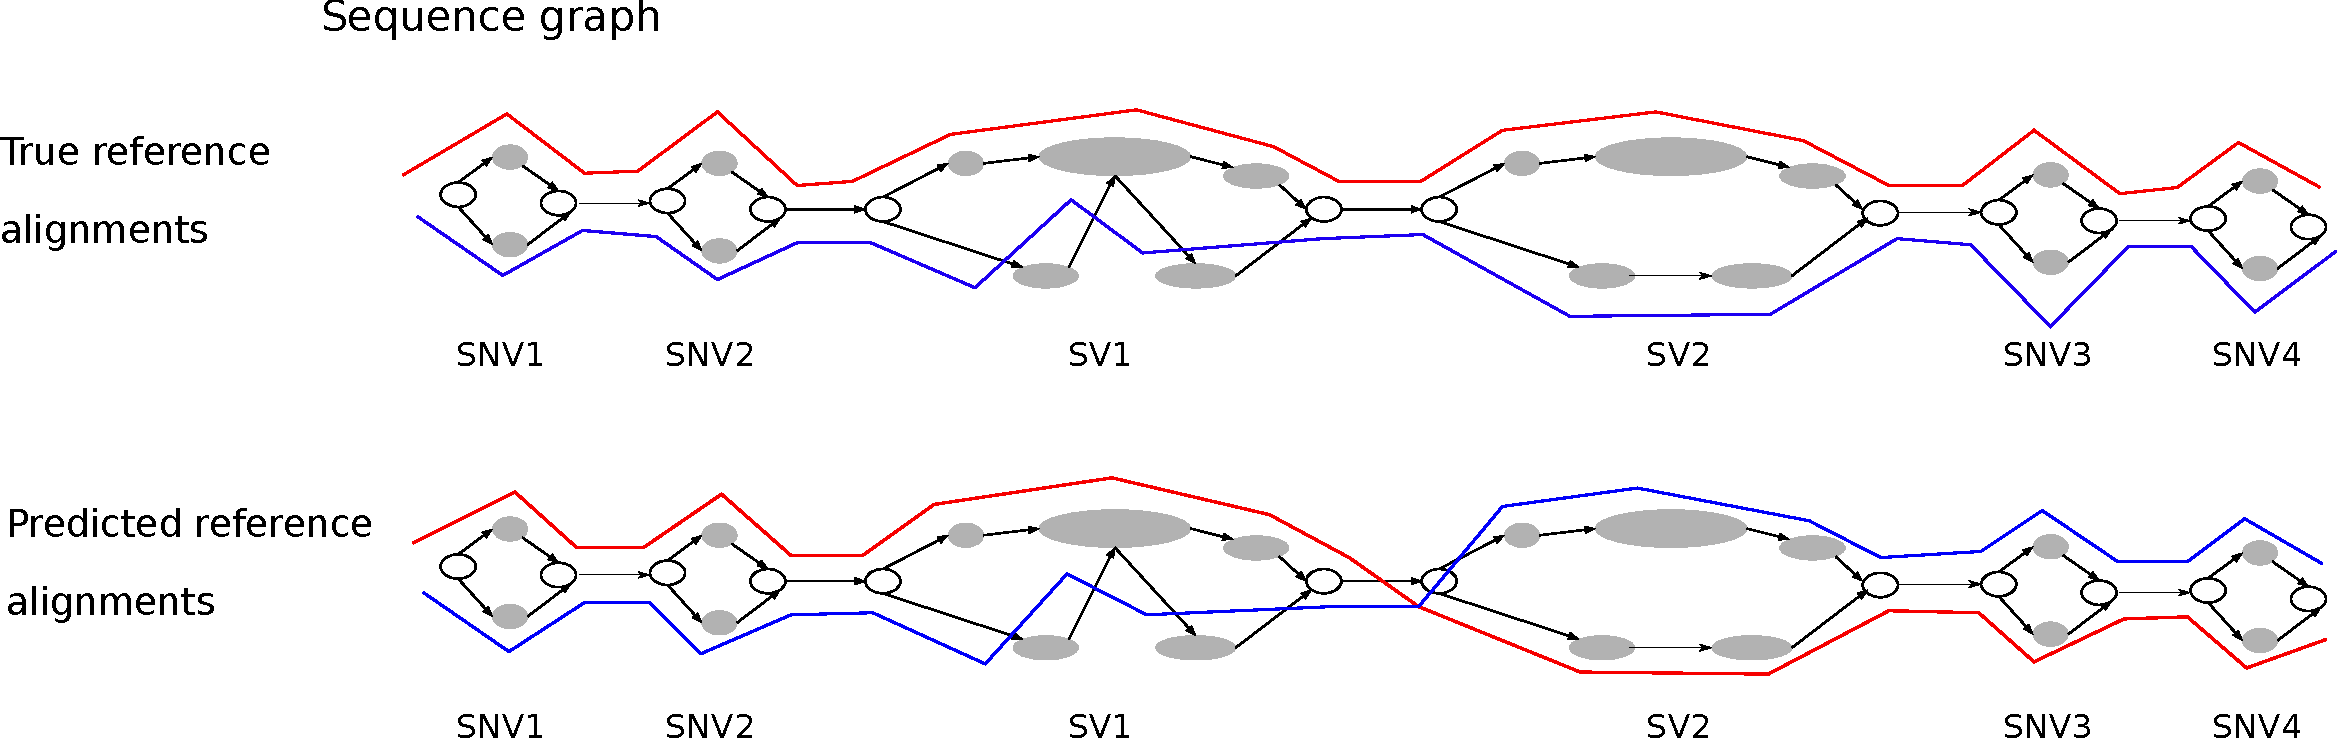
\includegraphics[width=\columnwidth]{evaluation.pdf}
\caption{For a subgraph of $G_s$, this example shows the true (top) and predicted (bottom) versions of two haplotype alignments (red and blue) through a series of bubbles. When comparing the correspondingly-colored lines between the two versions, we see one switch between SV1 and SV2: the prediction contains one switch error. 
Six bubbles have been phased, for a total of five phase connections between consecutive bubbles. Therefore, the phasing error rate is 1/5.}
\label{fig:evaluation}
\end{figure}

\subsection{Pipeline implementation}
\textit{Sequence graph}.
The first step in our pipeline is to perform error correction on the Illumina data by using BFC \citep{li2015bfc}, which, in our experience, retains heterozygosities well for diploid genomes.
BFC is used with default parameters and provided with a genome size of 12.16\,Mbp.
The second step is to generate a sequence graph that includes heterozygosity information.
To construct such a graph, we first construct the assembly graph by using a modified version of SPAdes v3.10.1 \citep{bankevich2012spades}.
We modify the original SPAdes to skip the bubble removal step and retain the heterozygosity information in the graph, and run it with default parameters plus the \texttt{{-}{-}only-assembler} option.
It uses the short Illumina reads to generate a De~Bruijn-based assembly graph without any error correction.
We then convert the assembly graph to a bluntified sequence graph using VG \citep{garrison2017sequence}.
After graph simplification, the resulting sequence graph has 158,567 nodes and 190,767 edges.

\textit{Bubble detection}. In the next stage, we use VG's snarl decomposition algorithm \citep{paten2017superbubbles} to detect the regions of heterozygosity, or \textit{snarls}, in the sequence graph. This results in 29,071 bubbles.
% and 58,183 total alleles of bubbles. 
% \todo{So there must be bubbles with only one allele since $29095\cdot 2= 58190$. How many multi-allelic bubbles are there?}.

\textit{PacBio Alignments}. After bubble detection, we align different coverage levels (10$\times$, 20$\times$ and 30$\times$) of long read PacBio data to the generated sequence graph using GraphAligner\footnote{\url{https://github.com/maickrau/GraphAligner}}.
% For efficient alignment of PacBio reads, we use a seed-based approach.
This resulted in 21,868, 43,459 and 73,129 PacBio alignments for input coverages of $10\times$, $20\times$ and $30\times$, respectively.

\textit{Bubble ordering}. To obtain an ordering of bubbles, we perform \textit{de novo} assembly using Canu v1.5 \citep{koren2017canu} on each PacBio dataset.
As suggested by \cite{giordano2017novo}, we use Canu v1.5 with the following parameter values: \texttt{corMhapSensitivity=high,} \texttt{corMinCoverage=2,} \texttt{correctedErrorRate=0.10,}\\
\texttt{minOverlapLength=499,} \texttt{corMaxEvidenceErate=0.3}.
Next, we align these Canu contigs to the sequence graph to obtain the bubble ordering, which we define as the sequence of bubbles encountered by each aligned contig.
Note that we use Canu solely for bubble ordering.
In this paper, we restrict ourselves to phasing bubbles only in unique, non-repetitive regions.
We detect repetitive bubbles based on the coverage depth of the PacBio alignments and remove them from downstream analyses.
The coverage depth threshold used is 1.67 times the average coverage.
This results in 148, 80, and 71 bubble chains, and 26,576, 27,556 and 27,741 bubbles, at coverages of $10\times$, $20\times$, and $30\times$ respectively.

% \todo{What is the definition of ``ordered bubble''? How many bubble chains and how many bubbles per chain on average?} 

\textit{Graph-based phasing}. For each of the coverage conditions, we take as input the ordered bubbles, the long-read PacBio alignments and the sequence graph, and solve the gMEC problem by assuming constant weights in the weight matrix $\mathcal{W}$.
The optimal bipartition is computed via backtracing and the final haplotigs are generated by concatenating the node labels of the two optimal paths.
These steps have been implemented in our WhatsHap software as a subcommand \texttt{phasegraph}\footnote{Presently this functionality resides in the \texttt{MAV} branch, which will be merged to the \texttt{master} branch in the near future and will be part of future WhatsHap releases.}.
\subsection{Running Falcon Unzip}
The main goal of this study is to measure the performance of phasing using a graph based approach, 
and, in particular, the quality of haplotypes at heterozygous sites achievable by using this method with low coverage PacBio data.
Therefore, we compared our graph-based approach to the state-of-the-art contig based phasing method Falcon Unzip, which also generates diploid assemblies.

The Falcon Unzip \citep{chin2016phased} algorithm first constructs a string graph composed of ``haploid consensus'' contigs, with bubbles representing structural variant sites between homologous loci. 
Sequenced reads are then phased and separated for each haplotype on the basis of heterozygous positions. 
Phased reads are finally used to assemble the backbone sequence (primary contigs) and the alternative haplotype sequences (haplotigs). 
The combination of primary contigs and haplotigs constitutes the final diploid assembly, which includes phasing information dividing single-nucleotide polymorphisms and structural variants between the two haplotypes.

We ran Falcon Unzip using the parameters given in the official parameter guide\footnote{http://pb-falcon.readthedocs.io/en/latest/parameters.html}.
We tried to run Falcon Unzip for lower coverages of 10$\times$ and 20$\times$, but it did not generate output in these cases (and we assume it is not designed for such low coverages).
Therefore, we only ran Falcon Unzip for 20$\times$ PacBio coverage.
Primary contigs and haplotigs were polished using the Quiver algorithm and corrected for SNPs and indels using Illumina data via Pilon, with the parameters ``\texttt{{-}{-}diploid}'' and ``\texttt{{-}{-}fix all}'' \citep{walker2014pilon}.
% To compare the Falcon Unzip haplotigs to the true references, we align the haplotigs produced by Falcon Unzip to our sequence graph and then 
% compared these aligned haplotigs to the true reference alignments through the bubbles.

\subsection{Assembly performance assessment}
To evaluate the accuracy of the predicted haplotypes, we align reference assemblies of the two yeast strains SK1 and Y12 \citep{yue2017contrasting} to the sequence graph.
% In doing so, first, we obtain the true references based on previously generated assemblies of two yeast strains SK1 and Y12 using high coverage PacBio data \citep{yue2017contrasting} and, second, we align these references to the sequence graph.
We emphasize that these reference assemblies are only used for evaluation purposes and are not a part of our assembly pipeline.
We use the following performance measures for the evaluation of diploid assemblies:

\textit{Phasing error rate}. Over the yeast genome, we compare the different diploid assemblies with the ground truth haploid genomes of SK1 and Y12.
As with the reference assemblies, we align the haplotigs produced by Falcon Unzip to our sequence graph.
For each phased bubble chain, the predicted haplotype is expressed as a mosaic of the two true haplotypes, minimizing the number of switches. 
This minimum then gives the number of switch errors.
% Note that the second predicted haplotype is exactly the complement of the first one, due to only considering heterozygous sites, and so does not have to be considered. \todo{But that's only true for bi-allelic loci, right? What happens at mulit-allellic loci?}
The phasing error rate is defined as the number of switch errors divided by the number of phased bubbles.
Figure~\ref{fig:evaluation} illustrates this calculation for a toy example.  The top panel shows the true references aligned to the sequence graph. At the bottom, predicted haplotypes (from Falcon Unzip or our graph-based approach) are aligned to the graph.
Comparing the true and predicted haplotypes, we see one switch between SV1 and SV2, which means that the switch error count is one. 
The number of phase connections between consecutive bubbles is five and the resulting switch error rate for this example is 1/5.

\textit{Average Percent Identity}. We consider the best assignment of each haplotig to either of the two true references, obtained by aligning the haplotig to the references.
For each whole diploid assembly, we compute the average of the best-alignment percent identities over all haplotigs. 

\textit{Assembly contiguity}. We assess the contiguity of the assemblies by computing the N50 of haplotig size.

\textit{Assembly completeness}. We consider two assembly completeness statistics: first, the total length of haplotigs assembled by each method, and second, the total number of unphased contigs.

% \begin{center}
\begin{table}[!ht]
\centering
\begin{tabular}{ |l|c|c|c| } 
 \hline
 Statistics & PacBio & Graph-based  & Falcon Unzip \\ 
 & coverage &  approach &  \\ 
  \hline
  \multicolumn{4}{|c|}{Diploid assemblies Quality}\\
  \hline
 Average Identity[\%] & 10$\times$& 99.50 & \textemdash\\
   & 20$\times$& 99.61  &\textemdash\\
   & 30$\times$& 99.80 &99.4 \\
 Phasing error rate[\%] & 10$\times$& 2.5 & \textemdash\\
   & 20$\times$& 1.5  &\textemdash\\
   & 30$\times$& 0.7 & 3.8 \\
  \hline
  \multicolumn{4}{|c|}{Contiguity}\\
  \hline
   N50 haplotig size [bp]& 10$\times$& 40k &\textemdash\\
   & 20$\times$& 42k &\textemdash\\
   & 30$\times$& 43k &32k\\ 
     \hline
  \multicolumn{4}{|c|}{Completeness}\\
  \hline
  Haplotig size [Mbp] & 10$\times$& 20.7 &\textemdash\\
   & 20$\times$& 21.1 &\textemdash\\
   & 30$\times$& 23.9 &16.6\\
   \# Unphased contigs  & 10$\times$& 2 &\textemdash\\
   & 20$\times$& 2 &\textemdash\\
   & 30$\times$& 2 &77\\
 \hline
\end{tabular}
\\[10pt]
 \caption{Comparison of two phasing methods, Falcon Unzip and our graph-based approach, at different PacBio coverage levels. For computing the ``haplotig N50'', we only consider those portions of a contig for which two haplotypes are available, i.e.\ those regions where Falcon reports both a primary contig and an alternative haplotig.
 For ``haplotig size'', we sum the length of contigs on both haplotypes (``primary contigs'' plus ``haplotigs'' in terms of Falcon's output), so the target size is twice the genome size (24.3Mbp in case of yeast).}
\label{table:graph_unzip}
\end{table}
% \end{center}
\section{Results}
In this section, we present the results of our analysis of the diploid assemblies generated by our method and by Falcon Unzip on the data sets described above.

\textit{Coverage analysis}. To discover a cost-effective method for assembling a diploid genome, we consider PacBio datasets that vary in terms of coverage---specifically, 10$\times$, 20$\times$ and 30$\times$ coverage are considered.
One of the primary aims of our study is to compare two approaches---the graph-based approach we implemented and the contig-based phasing done by Falcon Unzip. In doing so, we quantify the agreement between the diploid assemblies generated by both methods and the true references.
Table \ref{table:graph_unzip} shows the assembly performance statistics for both of these methods.
In order to assess the accuracy of the competing diploid assemblies, we compute the phasing error rate and the average percent identity at different PacBio coverages.
For the graph-based approach, we observe that as we increase the long read coverage from 10$\times$ to 30$\times$, the average identity of haplotigs increases from 99.5\% to 99.8\% and 
the phasing error rate decreases from 2.5\% to 0.7\%. In contrast, Falcon Unzip produces haplotigs with an average identity of 99.4\% and phasing error rate of 3.8\% at 30$\times$ coverage. 
Overall, comparing the agreement between the graph-based approach (at 10$\times$ coverage) and Falcon Unzip (at 30$\times$ coverage) to the true references, our graph-based approach delivers better haplotigs with respect to all measures reported in Table~\ref{table:graph_unzip}.
We believe that one reason for this is that we use an Illumina-based graph as a backbone.
Furthermore, optimally solving the gMEC formulation of the phasing problem most likely contributes to generating accurate haplotigs.
Overall, our analysis supports the conclusion that our approach delivers accurate haplotype sequences even at a long read coverage as low as 10$\times$.

To analyse the effect of different coverages of the Illumina short-read datasets on the quality of our haplotigs, we went back to the original, high coverage Illumina dataset (which we had been using downsampled to 50$\times$ coverage) and downsampled it to 100$\times$ coverage, i.e.\ twice the amount of reads used above.
We observed that increasing the coverage did not have a drastic effect on the quality of haplotigs.
The average phasing identity rose to 99.81\% and the total haplotig size was 23.9\,Mbp, which is virtually identical to the results for 50$\times$ as reported in Table~\ref{table:graph_unzip}.

\begin{figure*}[t!]
\begin{center}
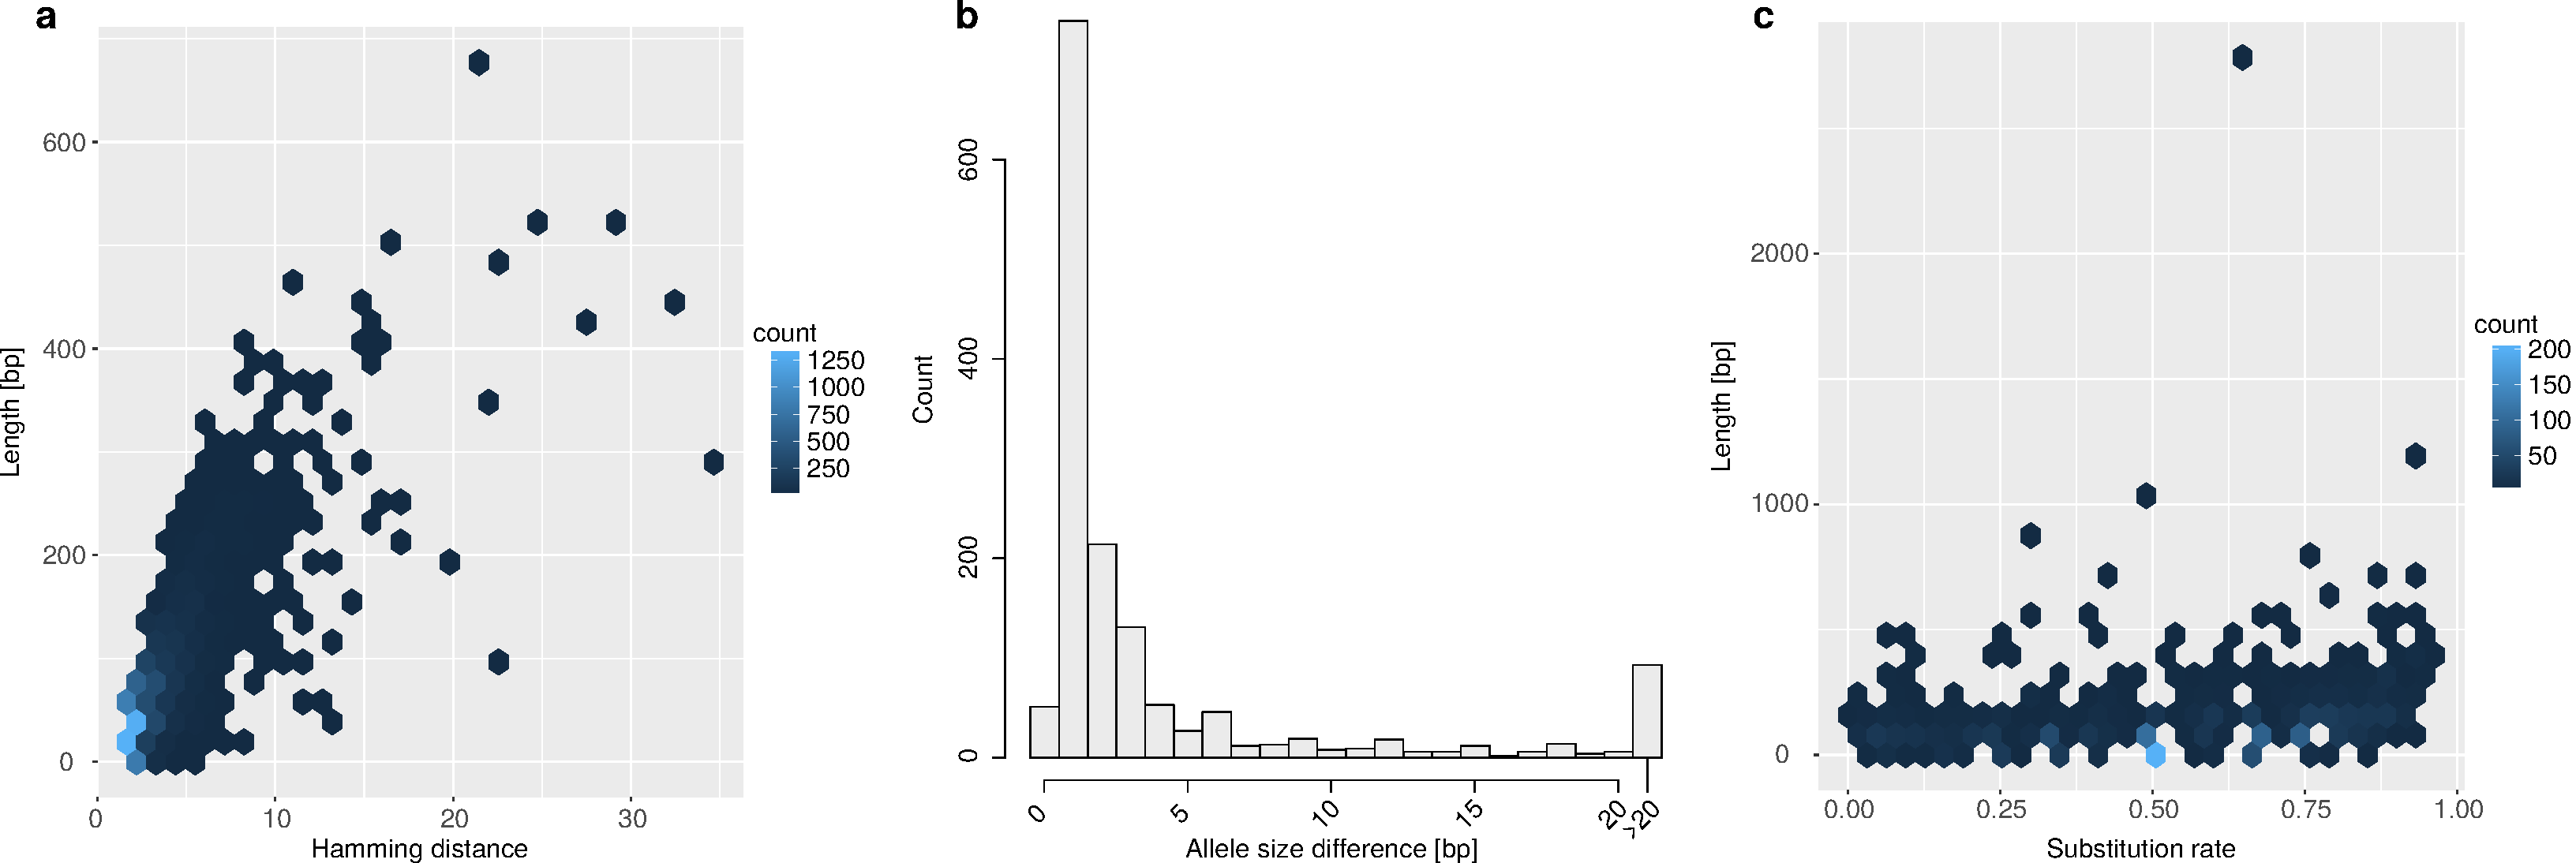
\includegraphics[width=\textwidth]{bubble-breakdown}%
\end{center}
\caption{Structural variation analysis of phased bubbles from our graph-based approach.
a: Joint distribution of allele length and Hamming distance, for pure substitutions.
b. Distribution of size difference between the two alleles, for mixed bubbles and indels. 
Pure substitutions always have a size difference of 0, and are not included in the figure.
c. Joint distribution of the length of the longer allele and the substitution rate, for mixed bubbles.
With a higher substitution rate, the bubble has more substitutions, and with a lower rate more indels.
}
\label{fig:bubble_breakdown}
\end{figure*}
With an increase in average PacBio coverage from 10$\times$ to 30$\times$, the haplotype contiguity achievable by using our approach improves from 40\,kbp to 43\,kbp.
By way of comparison, Falcon Unzip delivers haplotigs with a N50 length of 32\,kbp at the same coverage level. This highlights the fact that our approach generates more contiguous haplotypes compared to Falcon Unzip.
In terms of haplotype completeness, our approach yields diploid assemblies of length 20.7\,Mbp, 21.1\,Mbp and 23.9\,Mbp at average PacBio coverages of 10$\times$, 20$\times$ and 30$\times$ respectively.
At coverage 30$\times$, Falcon Unzip delivers a total assembly size of 16.6\,Mbp, while the total length of both haplotypes of the pseudo-diploid yeast genome is 24.3\,Mbp.
Our approach therefore delivers more complete haplotypes at a long-read coverage of 10$\times$ compared to Falcon Unzip at a coverage of 30$\times$.
There are 2 haplotigs that are not phased by our approach; this is due to the lack of heterozygosity over those regions.
In comparison, there are 77 (out of 123) contigs that are not phased by Falcon Unzip.
% We believe that the haplotig completeness and contiguity using the graph-based approach is mainly derived from aligning PacBio reads to the sequence graph, and additionally performing bubble calling and phasing them (as illustrated in Figure~\ref{fig:ex_graph_approach}).
In summary, our graph-based approach delivers complete and contiguous haplotype sequences even at a relatively low coverage of 10$\times$.

\textit{Bubble characterization}.
We attempted to characterize the nature of the heterozygous genomic variation encoded in the phased bubbles.
There are 25,033 bi-allelic bubbles phased by our approach when using 30$\times$ coverage PacBio data.
Of these bubbles, there are 15,293 for which both allele sequences have a length of at most 1\,bp, out of which 15,258 are single base pair substitutions (SNVs) and 35 are 1\,bp indels.
The remaining 9,740 bubbles either encode two or more small variants or more complex differences.
To differentiate these cases, we computed an alignment between the two allele paths and refer to those bubbles for which the alignment contains only substitutions but no indels as ``pure substitutions''.
Figure~\ref{fig:bubble_breakdown}a shows the joint distribution of length and (Hamming) distance for these pure substitution bubbles.
This analysis reveals, on the one hand, that many longer pure substitutions have a low distance and hence encode multiple SNVs and, on the other hand, that there also exists a population of more complex substitutions.
For the 1,489 bubbles not classified as pure substitutions, which we refer to as ``mixed bubbles'', Figure~\ref{fig:bubble_breakdown}b shows the absolute length difference between the two alleles.
While this difference is small for most bubbles, there are 93 bubbles with a length difference of 21\,bp or more.
To further elucidate the nature of the sequence differences, Figure~\ref{fig:bubble_breakdown}c presents the joint distribution of length of the longer allele and substitution rate, which is defined as the fraction of substitutions among all edit operations done to align the two sequences. (That is, a pure insertion or deletion has a substitution rate of 0.)

% the x-axis represents the edit distance between the two allele (haplotype) paths,
% % \todo{I wouldn't call this type and talk of edit distance right away. Confusing otherwise.} 
% and the y-axis represents the maximum length from these two haplotype sequences for each bubble.
% % The structural variant type for each bubble is determined by calculating the edit distance between the two allele (haplotype) paths, and the maximum variant size is calculated by considering the maximum length from these two haplotype sequences.
% The color of each point in the plot indicates the number of corresponding bubbles.
% Using our approach, in Figure~\ref{fig:sv_scatter}, we observe that 17,733 bubbles (out of 29,071) are at a bottom left corner with an edit distance of 1 bp, indicating that the bubbles describe SNVs or 1 bps indels. 
% There are a few points that lie on the diagonal (i.e. with one edit per base in the longest allele), which represent larger indels.
% % \todo{Also below 20bp, right?}.
% The points along the vertical line and those in between vertical and diagonal of the plot represent the bubbles containing SNPs or indels that are close to each other and that end up being contained in a single bubble.
% Furthermore, we see that some points represent larger and more complex variation.
% Overall, the distribution of phased bubbles in the plot indicates that the graph-based approach using both Illumina and PacBio data can phase both small and large structural variants.

% Taken together, the above analysis shows that our graph-based approach delivers better diploid assemblies even at lower PacBio coverages.
% In addition, the graph-based approach helps to detect and phase larger structural variants present in the diploid genomes.

% \begin{figure}[t!]\centering
% \includegraphics[width=\columnwidth]{falcon_bubbles.pdf}
% \caption{Structural variation analysis of phased bubbles from Falcon Unzip. The x axis and y axis show edit distance and maximum size for the two haplotype paths going through each bubble. The color shows the density of bubbles.}
% \label{fig:sv_scatter_falcon}
% \end{figure}


\section{Discussion}
The Falcon Unzip method \citep{chin2016phased} is based purely on PacBio reads, which exhibit a high error rate; it is therefore not suitable for lower coverages.
By using (costly) high coverage PacBio data, Falcon Unzip can generate good quality assemblies with an average haplotig identity of up to 99.99\% \citep{chin2016phased}.
% \todo{I do not see this number in the table above}. %, which is not the cost-effective way to solve the problem.
However, it follows a conservative approach for phasing genomic variants.
As sketched in Figure~\ref{fig:ex_graph_approach}, Falcon Unzip generates long primary contigs, but tends to phase them only partially.

To address the above problems, we have created a novel graph-based approach to diploid genome assembly that combines different sequencing technologies.
By using one technology producing shorter, more accurate reads, and a second technology delivering long reads, we produce accurate, complete and contiguous haplotypes. 
Our method also provides a cost-effective way of generating high quality diploid assemblies.
By performing phasing directly in the space of sequence graphs---without flattening them into contigs in intermediate steps---we can phase large structural variants, which is not possible using linear approaches. 
We have tested our approach using real data, in the form of a pseudo-diploid yeast genome, and we have shown that we deliver accurate and complete haplotigs.
Furthermore, we have shown that we can detect and phase structural variants.

In this study, we restricted ourselves to phasing unique, non-repetitive regions of the genome.
As a next step, we plan to develop techniques for phasing repetitive regions as well.
Resolving repeats and polyploids phasing are closely related problems, as pointed out by \cite{Chaisson2017}.
Therefore, we will aim to solve heterozygous variants and repeats in a joint phasing framework, in order to obtain even more contiguous diploid genome assemblies that include both types of features.
The machinery we plan to develop for this purpose would also remove the need to run an external assembler (Canu) for bubble ordering.
Finally, our framework allows, in principle, for incorporating additional data from other sequencing technologies, such as chromatin conformation capture \citep{burton2013chromosome}, linked read sequencing \citep{weisenfeld2017direct}, and single-cell template strand sequencing (Strand-seq; \citealp{Porubsky2016}).
In previous studies on reference-based haplotyping, we have shown such integrative approaches to be very powerful when inferring chromosome-scale haplotypes \citep{porubsky2017dense,chaisson2017multi}; we believe similar results can be obtained for \textit{de novo} diploid genome assemblies.
Moreover, studying the biological implications of the phased structural variation we can now detect also constitute an exciting future research direction.

